\chapter{User Manual}
\settocdepth{chapter}
\label{appendix-user-manual}

\begin{center}
  \begin{figure}[ht!]
    \makebox[\textwidth]{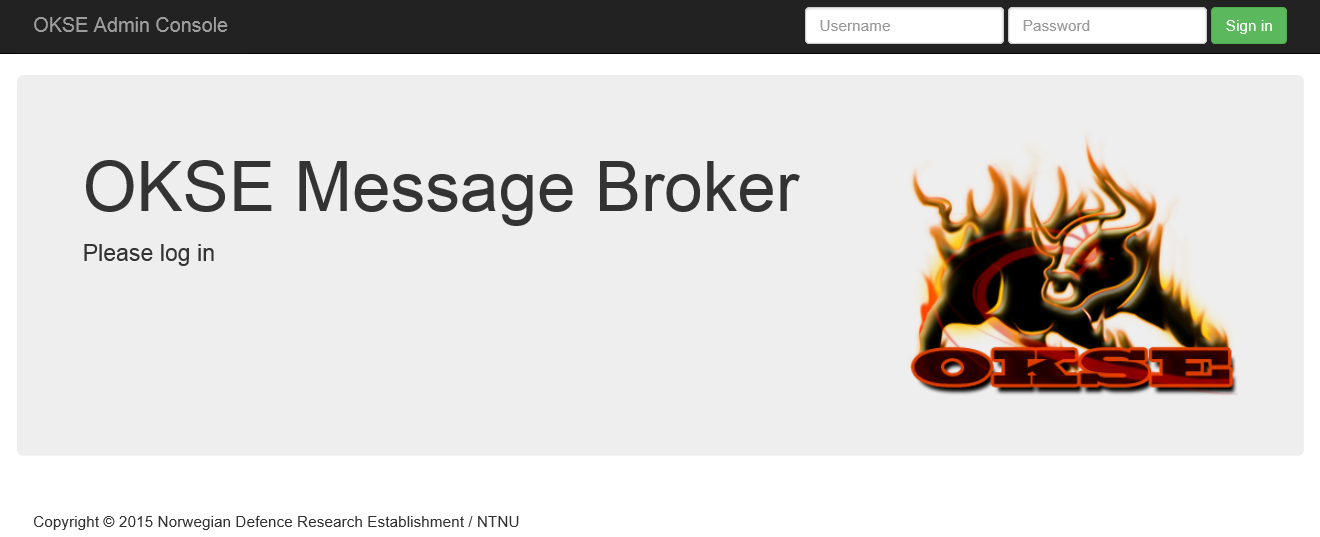
\includegraphics[width=\textwidth]{fig/oac/oac.png}}
    \caption{The OKSE Admin Console login page} 
    \label{fig:OKSE Admin Console login page}
  \end{figure}
\end{center}

\section{About}

This chapter contains instructions for installing and using the OKSE Message Broker. The intended users are primarily researchers working with collaborative networking. OKSE is open source, and licensed under the MIT license.

\section{Requirements}

OKSE Message Broker requires Java Runtime Environment (JRE) version 8 update 31 or newer. The broker is developed and tested exclusively with this version. The software is available for free from http://java.com\footnote{\url{http://www.oracle.com/technetwork/java/javase/downloads/jre8-downloads-2133155.html}}.

For the JRE to function properly, it must be added to the path variable. On UNIX-based systems, like Linux or OS X, it is done by the Java installer. On windows, open up a command line window (cmd.exe) and type in:
\begin{verbatim}
path %path%;<PATH-TO-JRE>
\end{verbatim}
Usually this can by done on Windows by entering:
\begin{verbatim}
path %path%;C:\ProgramData\Oracle\Java\javapath
\end{verbatim}
The variable can also be accessed and modified through the "Environmental variables" tab in the advanced system settings. The system should be possible to run on all platforms with JRE installed. 

In addition to JRE, OKSE requires a network connection to be able to send and receive messages. It does not however, require Internet on the connection. 

\section{Installation}
\label{Installation_okse}

The following sections describes how to download and run OKSE. Apart from JRE, no other additional configuration should be necessary.

\subsection{Download software}

Download the latest version of OKSE Message Broker from http://okse.fap.no/ or use the version provided with this document. The files can be placed at any location within the filesystem, as long as the user has write permission in the target folder. It's recommended that all files are placed in the same folder.

\subsection{Running the software}

\subsubsection{Using the start script}
Within the main folder of the software package, there are two scripts, \verb!start.bat! and \verb!start.sh!. The scripts will automatically try to detect where Java is installed and start the application.\\\\With Windows, the application can be started by double clicking \verb!start.bat!. This will bring up a console window with the application. To close the application, simply close the window.\\\\With Unix/Linux/OS X, the script should be run with a terminal. As there is a lot of different versions of Linux/Unix, consult the documentation of the distribution on how to do this.\\\\With OS X, the script can be started by following these steps:

\begin{enumerate}
\item Right click \verb!start.sh!
\item Select Open With $\rightarrow$ Other...
\item Go to utilities
\item Select Terminal.app (Select Enable: All Applications)
\end{enumerate}

\subsubsection{Using command line}

On UNIX-based systems and using cmd.exe on Windows, the broker is started by running these commands from the command line or terminal: 
\begin{verbatim}
cd <PATH-TO-OKSE>
java -jar okse.jar
\end{verbatim}

\noindent If the broker is going to be used for bigger files or a very high amount of messages, a higher memory limit should be set for Java. Note that it is not possible to set the memory limit higher than the amount of memory that is available: 

The following command changes the memory limit:

\begin{verbatim}
java -jar -Xms2048m -Xmx4096m okse.jar
\end{verbatim}
See section \ref{sec:inital-login} for information about accessing the administration panel.

\section{Configuration}

After the initial start up of OKSE Message Broker, a folder named \verb!config! is created in the same location as the .jar-file. This folder contains three configuration files with default configuration:

\begin{itemize}
\setlength{\itemsep}{0cm}%
\item okse.properties
\item log4j.properties
\item topicmapping.properties
\end{itemize}

\noindent See section \ref{sec:configuration_files} for detailed information about all the possible settings.

\section{Inital login}
\label{sec:inital-login}

After launching the application, the administrator interface will be reachable from the web browser. The default hostname, port and login information can be found below. If OKSE is hosted on a server, not that the host will be the domain/IP of the server.

\begin{itemize}
\setlength{\itemsep}{0cm}%
\item Default host and port for admin console: \verb!localhost:8080!
\item Default username and password: \verb!admin! and \verb!password!
\end{itemize}

\section{Admin Console}
The OKSE Admin Console provides information about OKSE and it is operation environment. It also gives access to configure OKSE. The interface have information sorted in six panes, "Main", "Topics", "Subscribers", "Statistics", "Configuration" and "Logs".

\clearpage

\subsection{The main pane}
\begin{center}
  \begin{figure}[ht!]
    \makebox[\textwidth]{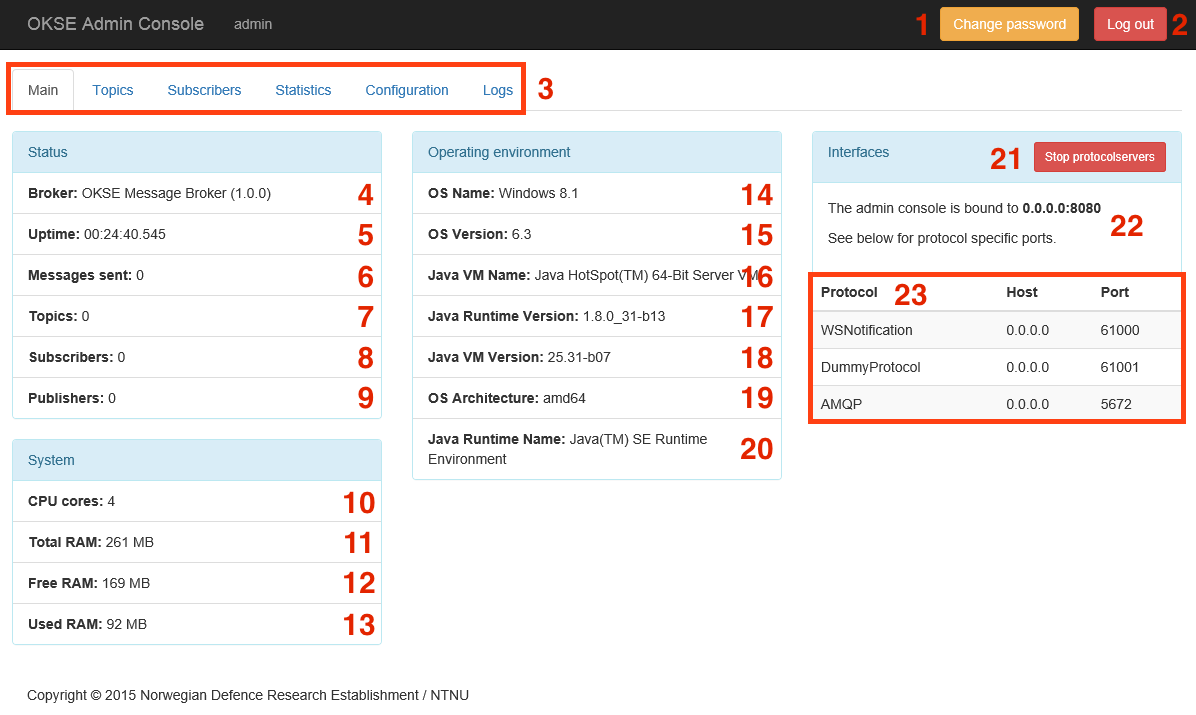
\includegraphics[width=\textwidth]{fig/oac/n/mainpane_n.png}}
    \caption{The OKSE Admin Console - Main pane} 
    \label{fig:OKSE Admin Console - Main pane}
  \end{figure}
\end{center}
\begin{enumerate}
\item Change the admin password
\item Log out from OKSE
\item Navigation bar with available pages
\item Version and name of broker
\item Time since the broker was started
\item Total number of sent messages
\item Total number of topics
\item Total number of subscribers
\item Total number of publishers
\item Amount of CPU cores in the host system
\item Total amount of RAM allocated to the Java Virtual Machine
\item Total amount of free RAM
\item Total amount of used RAM
\item Name of the operating system
\item Version of the operating system
\item Name of the Java VM
\item Version of the Java VM Runtime
\item Version of the Java VM
\item Architecture of the host system
\item Name of the Java VM Runtime
\item Stop/Start all the protocol servers
\item Information about the address and port for the admin UI
\item Address and port information for each protocol
\end{enumerate}

%The main pane is an overview of the broker's status, system, the operating environment as well as interfaces and ports that the different protocol servers are bound to. It's worth mentioning that the RAM reported is the memory available in the Java virtual machine. It is also possible to stop and start the protocol servers from the interface section. When the protocol servers are restarted, the statistics are reset.

\clearpage


\subsection{The topics pane}
\begin{center}
  \begin{figure}[ht!]
    \makebox[\textwidth]{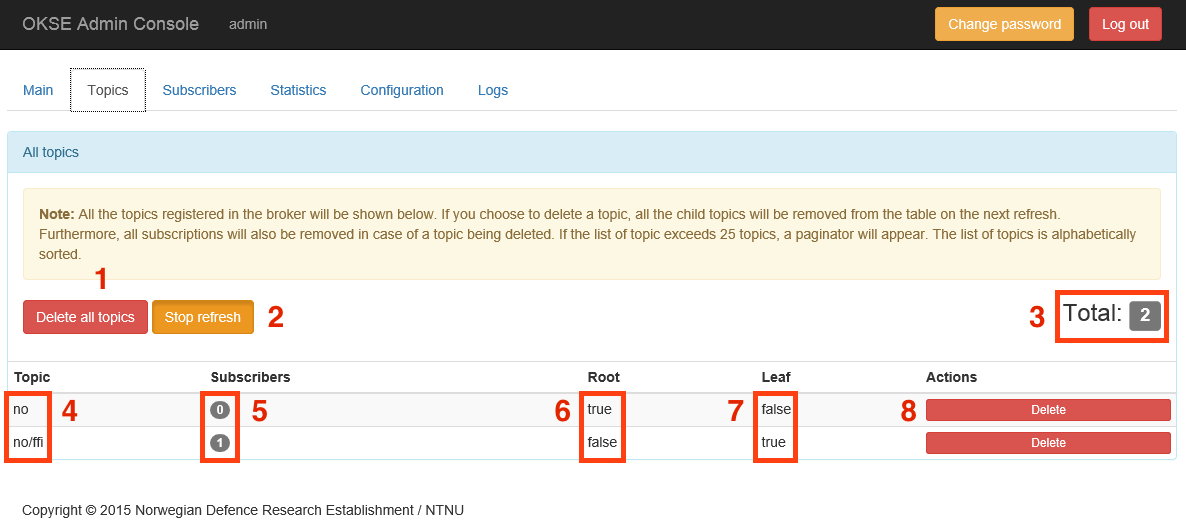
\includegraphics[width=\textwidth]{fig/oac/n/topicspane_n.png}}
    \caption{The OKSE Admin Console - Topics pane} 
    \label{fig:OKSE Admin Console - Topics pane}
  \end{figure}
\end{center}
\begin{enumerate}
\item Delete existing topics, cannot be recovered
\item Stop automatic refresh of the webpage
\item Total amount of topics
\item Name of the topic
\item Amount of subscribers
\item Is the topic a root node?
\item Is the topic a leaf node?
\item Delete the topic on this line
\end{enumerate}

%The "Topics" pane contains all the registered topics in OKSE. For each topic it is possible to see how many clients are subscribing to the topic (---comment about xpath not being subscribers??---). It is also possible to delete all topics or a specific topic. The 'Stop refresh'-button stops the automatic refreshing of the topic list. This might be useful when a lot of new topics are generated, to avoid the list updating constantly.

\clearpage

\subsection{The subscribers pane}
\begin{center}
  \begin{figure}[ht!]
    \makebox[\textwidth]{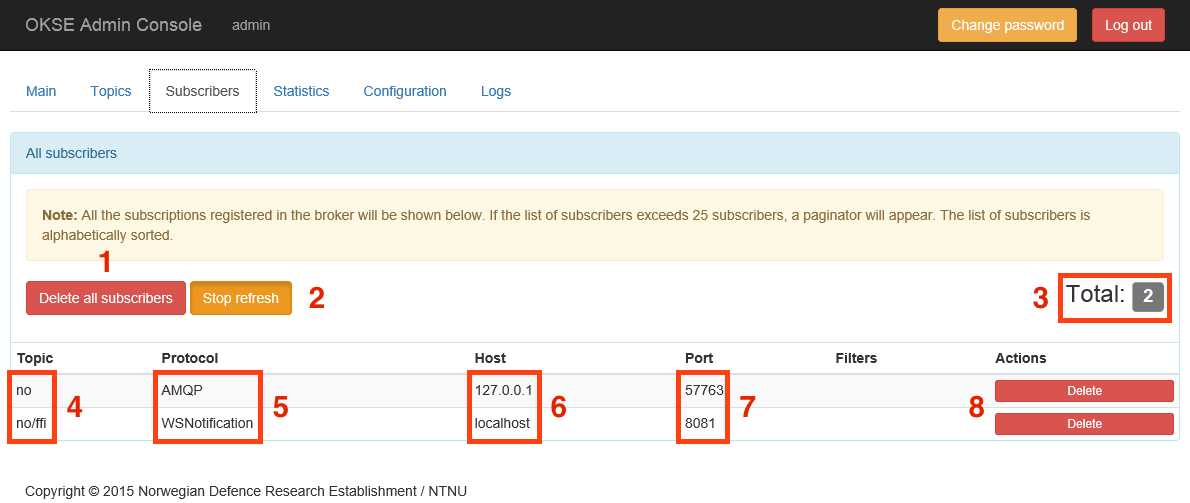
\includegraphics[width=\textwidth]{fig/oac/n/subscriptionspane_n.png}}
    \caption{The OKSE Admin Console - Subscriptions pane} 
    \label{fig:OKSE Admin Console - Subscriptions pane}
  \end{figure}
\end{center}
\begin{enumerate}
\item Delete all existing subscribers
\item Stop automatic refresh of the webpage
\item Total amount of subscribers
\item The topic that the subscriber is subscribed to
\item The protocol in use by the subscriber
\item The port in use by the subscriber
\item Delete the subscriber on this line
\end{enumerate}
%The subscribers pane lists all the subscribers (hosts). It also lists which protocols the different subscribers are using, on which port, and if any filters are specified. One or all of the users can be deleted, denoted as unsubscribe in WSN and disconnect in AMQP. The 'Stop refresh'-button stops the automatic refreshing of the subscription list. This might be useful when there are many clients subscribing and/or unsubscribing, to avoid the list updating constantly.

\clearpage

\subsection{The Statistics pane}
\begin{center}
  \begin{figure}[ht!]
    \makebox[\textwidth]{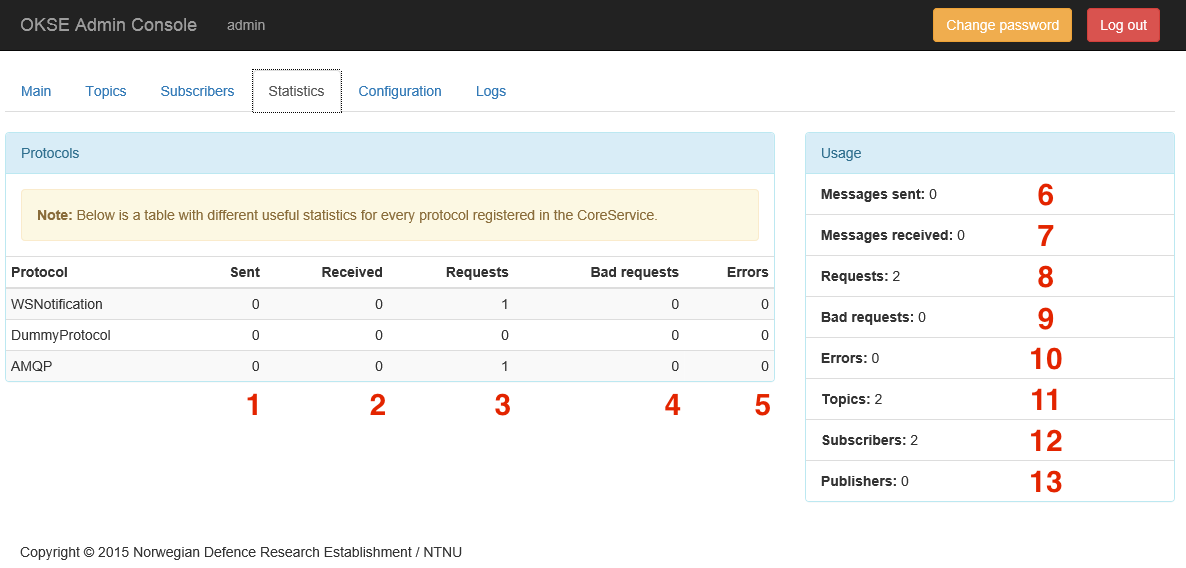
\includegraphics[width=\textwidth]{fig/oac/n/statisticspane_n.png}}
    \caption{The OKSE Admin Console - Statistics pane} 
    \label{fig:OKSE Admin Console - Statistics pane}
  \end{figure}
\end{center}
\begin{enumerate}
\item Amount of messages sent by each protocol
\item Amount of messages received by each protocol
\item Amount of request to each protocol
\item Amount of bad request to each protocol
\item Amount of errors received on each protocol
\item Total amount of messages sent through the system
\item Total amount of messages received by the system
\item Total amount of requests handled by the system
\item Total amount of bad requests received by the system
\item Total amount of errors received by the system
\item Total amount of topics currently handled by the system
\item Total amounf of subscribers currently handled by the system
\item Total amount of publishers currently handled by the system
\end{enumerate}
%The Statistics pane provides a list of protocol servers with statistics per protocol and total usage. "Sent" denotes the amount of messages sent on the different protocols. "Received" denotes the amount of messages received on the current protocol. "Requests" are the total amount of requests on the protocol. The WSN protocol server requests are subscribe requests, messages sent to the broker, publisher registration, and attempts to access an endpoint address. AMQP requests are socket connections to the broker and messages sent to the broker. Bad requests on WSN appear whenever a request fails to complete correctly. AMQP does not count "Bad requests". Errors are counted on WSN when OKSE attempts to send a message, but are unable to reach the subscriber. In AMQP, errors are noted whenever someone attempts to connect to OKSE on AMQP's port, but the connection is not accepted. The usage panel shows the total statistics over all the protocols.

\clearpage

\subsection{The Configuration pane}
\begin{center}
  \begin{figure}[ht!]
    \makebox[\textwidth]{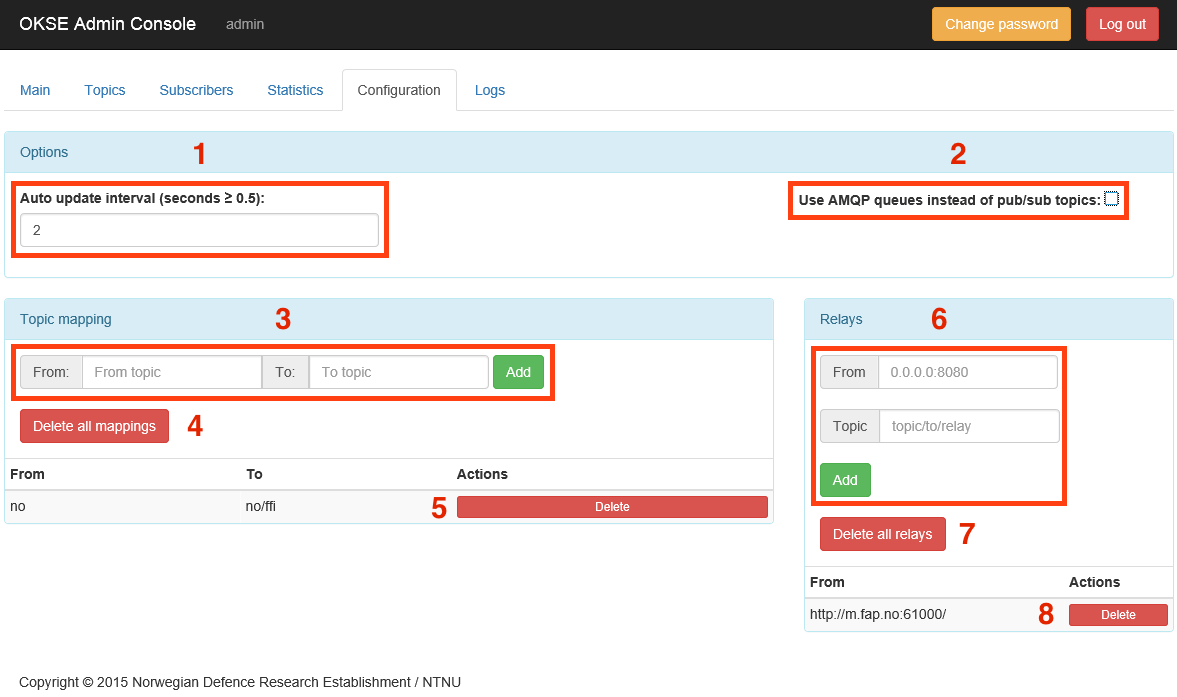
\includegraphics[width=\textwidth]{fig/oac/n/configurationpane_n.png}}
    \caption{The OKSE Admin Console - Configurations pane} 
    \label{fig:OKSE Admin Console - Configurations pane}
  \end{figure}
\end{center}
\begin{enumerate}
\item The admin panel update interval
\item Toggle the use of queue/topic behaviour in AMQP
\item Map one topic to another.
\item Delete all existing topic mappings
\item Delete the topic mapping on this line
\item Set up a relay to another WSN compliant broker
\item Delete all exisiting relays
\item Delete the relay on this line
\end{enumerate}
%The Configuration pane has three sections; options, topic mapping and relays. The option section allows changing the update automatic refresh interval on the site. It is not recommended that this is set lower than 0.5 seconds. The "Use AMQP queues instead of pub/sub topics" changes the queue semantics of AMQP.

%In the topic mapping section one can manually map from one topic to another one. The mapping of topics is a simplex action, that is, an action that is one-way. If a mapping is made between topic A and B, messages sent to A will also be forwarded to topic B. Messages sent to topic B will not be forwarded to topic A. Mapping from and to unregistered topics are allowed, and causes the topics to be generated.

%The relays section enables the addition of an instance of the system as a relay node (child relay) to another instance or WSN broker. The function is enabled by entering the address and the port the other broker is running on. The topic input is optional, and provides the opportunity to relay a specific topic by typing in the name of it. If the field is left empty, everything is relayed. When adding a relay, a WSNotification subscription is created. There are some bounds to the relay, to avoid infinite looping of messages. There are restrictions on localhost, 127.0.0.1, 0.0.0.0 and interfaces on the running instance of OKSE.

\clearpage

\subsection{The Logs pane}
\begin{center}
  \begin{figure}[ht!]
    \makebox[\textwidth]{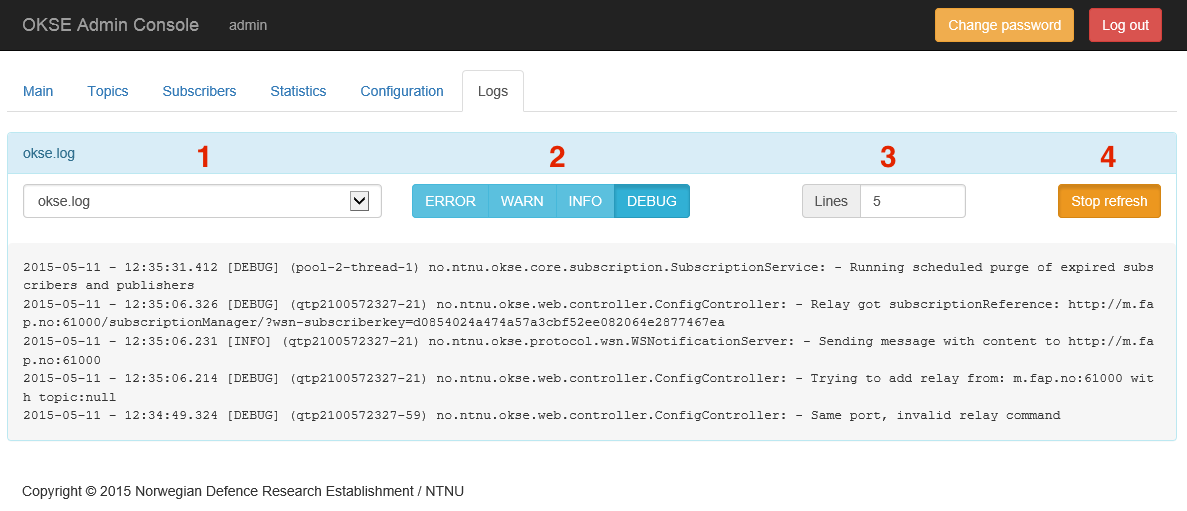
\includegraphics[width=\textwidth]{fig/oac/n/logpane_n.png}}
    \caption{The OKSE Admin Console - Logs pane} 
    \label{fig:OKSE Admin Console - Logs pane}
  \end{figure}
\end{center}
\begin{enumerate}
\item Choose the desired logfile
\item Select the loglevel
\item Enter the amount of lines of log
\item Stop automatic refresh of the webpage
\end{enumerate}
%The main feature of the "Logs" pane is the large text area, providing all of the information printed from the application. Logging is separated into 4 levels, "ERROR", "WARN", "INFO" and "DEBUG". The "DEBUG" level shows the full set of messages printed during system runtime. "INFO" prints messages that are meant to show the progress and events happening in the application. The "WARN" level prints messages that might potentially lead to system failure. Finally, "ERROR" shows events which has caused a failure in the system. There are one button for each of the message types, allowing the user to filter out information. The "Lines" area, lets the user decide how many lines of information that are displayed. Finally, the "Stop refresh" buttons stops new messages from showing up in the text-area.

\clearpage

\section{Configuration files}
\label{sec:configuration_files}
OKSE has three configurations files. The main configuration file is the okse.properties file. The two other files are log4j.properties, and topicmapping.properties for log- and topic mapping configuration. The following sections describe the default behaviour, defined by each of the files.

\subsection{okse.properties}
\label{subsec:configuration_files-okse.properties}
 
This is the main configuration file of the system. Below is a list of the possible settings, and a description.

\begin{description}
\setlength{\itemsep}{0cm}%
  \item[sprint.application.name] \hfill \\
  Application name to be displayed in the Admin Console \hfill \\ Default: \verb!OKSE Message Broker!
  \item[server.port] \hfill \\
  Tells Jetty which port the Admin Console should listen to \hfill \\ Default: \verb!8080!
  \item[ADMIN\_PANEL\_HOST] \hfill \\
  The host the Admin Console should listen to \hfill \\ Default: \verb!0.0.0.0!
  \item[CACHE\_MESSAGES] \hfill \\
  Tells OKSE if it should cache messages \hfill \\ Default: \verb!true!
  \item[BROADCAST\_SYSTEM\_MESSAGES\_TO\_SUBSCRIBERS] \hfill \\
  Tells OKSE if system messages should be broadcasted to all subscribers \hfill \\ Default: \verb!false!
  \item[ENABLE\_WSNU\_DEBUG\_OUTPUT] \hfill \\
  Tells OKSE if it should log WSNU \hfill \\ Default: \verb!false!
  \item[DEFAULT\_SUBSCRIPTION\_TERMINATION\_TIME] \hfill \\
  Tells OKSE what the subscription termination time should be \hfill \\ Default: \verb!15552000000!
  \item[DEFAULT\_PUBLISHER\_TERMINATION\_TIME] \hfill \\
  Tells OKSE what the publisher termination time should be \hfill \\ Default: \verb!15552000000!
  \item[TOPIC\_MAPPING] \hfill \\
  Tells OKSE the path to the topic mapping configuration file \hfill \\ Default: \verb!config/topicmapping.properties!
  \item[WSN\_HOST] \hfill \\
  Tells OKSE what host WSNotificanServer should listen to \hfill \\ Default: \verb!0.0.0.0!
  \item[WSN\_PORT] \hfill \\
  Tells OKSE what port WSNotificationServer should listen to \hfill \\ Default: \verb!61000!
  \item[WSN\_CONNECTION\_TIMEOUT] \hfill \\
  Tells OKSE what connection timeout to use with WS-Notification \hfill \\ Default: \verb!5!
  \item[WSN\_POOL\_SIZE] \hfill \\
   WSNotification http client thread pool used to queue outbound requests \hfill \\ Default: \verb!50!
   \item[WSN\_MESSAGE\_CONTENT\_ELEMENT\_NAME] \hfill \\
  Tells OKSE what name non-XML content should be wrapped in \hfill \\ Default: \verb!Content!
  \item[WSN\_USES\_NAT] \hfill \\
  Tells OKSE if it's hosted behind NAT/Port forwarded network \hfill \\ Default: \verb!false!
  \item[WSN\_WAN\_HOST] \hfill \\
  Tells OKSE what host it's behind when using NAT \hfill \\ Default: \verb!test.doman.com!
  \item[WSN\_WAN\_PORT] \hfill \\
  Tells OKSE what port it's behind when using NAT \hfill \\ Default: \verb!61000!
  \item[DUMMYPROTOCOL\_HOST] \hfill \\
  Tells OKSE what host DummyProtocolServer should listen to \hfill \\ Default: \verb!0.0.0.0!
  \item[DUMMYPROTOCOL\_PORT] \hfill \\
  Tells OKSE what port DummyProtocolServer should listen to \hfill \\ Default: \verb!61001!
  \item[AMQP\_HOST] \hfill \\
  Tells OKSE what host AMQPProtocolServer should listen to \hfill \\ Default: \verb!0.0.0.0!
  \item[AMQP\_PORT] \hfill \\
  Tells OKSE what port AMQPProtocolServer should listen to \hfill \\ Default: \verb!5672!
  \item[AMQP\_USE\_QUEUE] \hfill \\
  Tells OKSE if AMQP should use the standard queue or the non-standard topic implementation \hfill \\ Default: \verb!false!
  \item[AMQP\_USE\_SASL] \hfill \\
  Tells OKSE if AMQP should use SASL \hfill \\ Default: \verb!true!
  \item[spring.resources.cache-period] \hfill \\
  Tells Spring what cache-period to set on HTTP-requests \hfill \\ Default: \verb!1!
  \item[spring.thymeleaf.suffix] \hfill \\
  Tells Spring what all Thymeleaf templates are suffixed with \hfill \\ Default: \verb!.html! 
   \item[spring.thymeleaf.mode] \hfill \\
  Tells Spring what type all Thymeleaf templates are \hfill \\ Default: \verb!HTML5!
   \item[spring.thymeleaf.encoding] \hfill \\
  Tells Spring what encoding to use on all Thymeleaf templates \hfill \\ Default: \verb!UTF-8!
   \item[spring.thymeleaf.content-type] \hfill \\
  Tells Spring what content-type all Thymeleaf templates should be returned with \hfill \\ Default: \verb!text/html! 
\end{description}
  
 \subsection{log4j.properties}
 \label{subsec:log4j.properties}
 
This is the configuration file for all the log files available for the system. See below for a detailed list of all possible settings, and their description.

\begin{description}

\setlength{\itemsep}{0cm}%
  \item[log] \hfill \\
  Default folder location for log files, relative to .jar file \hfill \\ Default: \verb!logs!
  \item[pattern] \hfill \\
  Default pattern to print log output in \hfill \\ Default: \verb!%d{yyyy-MM-dd - HH:mm:ss.SSS} [%p] (%t) %c: - %m%n!
   \item[maxLogFileSize] \hfill \\
  Max log file size, before log rotate \hfill \\ Default: \verb!5MB!
   \item[numberOfBackups] \hfill \\
  Max number of log files, before it purges old files \hfill \\ Default: \verb!10!
   \item[log4j.logger.no.ntnu.okse] \hfill \\
  Default log level for okse log messages \hfill \\ Default: \verb!DEBUG, OKSE!
  \item[log4j.logger.org.apache.qpid] \hfill \\
  Default log level for qpid log messages \hfill \\ Default: \verb!DEBUG, QPID!
  \item[log4j.logger.org.eclipse.jetty] \hfill \\
  Default log level for Jetty log messages \hfill \\ Default: \verb!INFO, JETTY!
  \item[log4j.logger.org.springframework] \hfill \\
  Default log level for Spring log messages \hfill \\ Default: \verb!INFO, SPRING!
  
  \item[log4j.appender.OKSE] \hfill \\
  Default appender to use for OKSE logs \hfill \\ Default: \verb!org.apache.log4j.RollingFileAppender!
  \item[log4j.appender.OKSE.File] \hfill \\
  Default log file to use for OKSE logs \hfill \\ Default: \verb!${log}/okse.log!
   \item[log4j.appender.OKSE.MaxFileSize] \hfill \\
  Default log file size to use for OKSE logs \hfill \\ Default: \verb!${maxLogFileSize}!
   \item[log4j.appender.OKSE.MaxBackupIndex] \hfill \\
  Number of backups for OKSE logs \hfill \\ Default: \verb!${numberOfBackups}!
   \item[log4j.appender.OKSE.layout] \hfill \\
  Pattern engine for OKSE logs \hfill \\ Default: \verb!org.apache.log4j.PatternLayout!
   \item[log4j.appender.OKSE.layout.conversionPattern] \hfill \\
  Default pattern to use for OKSE logs \hfill \\ Default: \verb!${Pattern}!

    \item[log4j.appender.SPRING] \hfill \\
  Default appender to use for SPRING logs \hfill \\ Default: \verb!org.apache.log4j.RollingFileAppender!
  \item[log4j.appender.SPRING.File] \hfill \\
  Default log file to use for SPRING logs \hfill \\ Default: \verb!${log}/spring.log!
   \item[log4j.appender.SPRING.MaxFileSize] \hfill \\
  Default log file size to use for SPRING logs \hfill \\ Default: \verb!${maxLogFileSize}!
   \item[log4j.appender.SPRING.MaxBackupIndex] \hfill \\
  Number of backups for SPRING logs \hfill \\ Default: \verb!${numberOfBackups}!
   \item[log4j.appender.SPRING.layout] \hfill \\
  Pattern engine for SPRING logs \hfill \\ Default: \verb!org.apache.log4j.PatternLayout!
   \item[log4j.appender.SPRING.layout.conversionPattern] \hfill \\
  Default pattern to use for SPRING logs \hfill \\ Default: \verb!${Pattern}!

  \item[log4j.appender.JETTY] \hfill \\
  Default appender to use for JETTY logs \hfill \\ Default: \verb!org.apache.log4j.RollingFileAppender!
  \item[log4j.appender.JETTY.File] \hfill \\
  Default log file to use for JETTY logs \hfill \\ Default: \verb!${log}/okse.log!
   \item[log4j.appender.JETTY.MaxFileSize] \hfill \\
  Default log file size to use for JETTY logs \hfill \\ Default: \verb!${maxLogFileSize}!
   \item[log4j.appender.JETTY.MaxBackupIndex] \hfill \\
  Number of backups for JETTY logs \hfill \\ Default: \verb!${numberOfBackups}!
   \item[log4j.appender.JETTY.layout] \hfill \\
  Pattern engine for JETTY logs \hfill \\ Default: \verb!org.apache.log4j.PatternLayout!
   \item[log4j.appender.JETTY.layout.conversionPattern] \hfill \\
  Default pattern to use for JETTY logs \hfill \\ Default: \verb!${Pattern}!
  
    \item[log4j.appender.QPID] \hfill \\
  Default appender to use for QPID logs \hfill \\ Default: \verb!org.apache.log4j.RollingFileAppender!
  \item[log4j.appender.QPID.File] \hfill \\
  Default log file to use for QPID logs \hfill \\ Default: \verb!${log}/qpid.log!
   \item[log4j.appender.QPID.MaxFileSize] \hfill \\
  Default log file size to use for QPID logs \hfill \\ Default: \verb!${maxLogFileSize}!
   \item[log4j.appender.QPID.MaxBackupIndex] \hfill \\
  Number of backups for QPID logs \hfill \\ Default: \verb!${numberOfBackups}!
   \item[log4j.appender.QPID.layout] \hfill \\
  Pattern engine for QPID logs \hfill \\ Default: \verb!org.apache.log4j.PatternLayout!
   \item[log4j.appender.QPID.layout.conversionPattern] \hfill \\
  Default pattern to use for QPID logs \hfill \\ Default: \verb!${Pattern}!

 \item[log4j.appender.stdout] \hfill \\
  Default appender to use for console output \hfill \\ Default: \verb!org.apache.log4j.ConsoleAppender!
   \item[log4j.appender.stdout.Target] \hfill \\
  Default target to use for console output \hfill \\ Default: \verb!System.out!
    \item[log4j.appender.stdout.layout] \hfill \\
  Pattern engine for console logs \hfill \\ Default: \verb!org.apache.log4j.PatternLayout!
   \item[log4j.appender.stdout.layout.conversionPattern] \hfill \\
  Default pattern to use for console logs \hfill \\ Default: \verb!${Pattern}!
  
 \end{description}
 
 \subsection{topicmapping.properties}
 \label{subsec:topicmapping.properties}
 
This is a configuration file for adding predefined topic mappings upon system initialization. To add predefined topic mappings, use the format from the example below. The example shows a simplex mapping and a duplex mapping. In the simplex mapping the first topic, no/ffi, is forwarded to nato/hq/info, but not the other way. In the duplex mapping, all messages received on each topic will be forwarded to the other.

\begin{verbatim}
# Simplex mapping
no/ffi=nato/hq/info

# Duplex mapping
no/test=com/test
com/test=no/test
\end{verbatim}
 
\section{Test clients}
\label{sec:test_clients}
As none of the protocols had any useful clients for testing, a JAR file is included for AMQP send and one for AMQP receive. Keep in mind that little time has been spent on these programs, and that they are only suitable for minor testing. The files can only be run from the command line with the arguments given below. Other tools where used in the testing of WSN, but the tools are owned by FFI and cannot be distributed any further, more information about this in appendix \ref{appendix-eula}. Note that these test clients do not reflect proper usage of the software, but are meant for test purposes.

\subsection{AMQP send}
\label{subsec:test_clients-amqp_send}
Provided in the project delivery is a folder named test-clients, within this folder, the file amqpsend.jar is located. The file takes three arguments.

\begin{description}
    \item[-a amqp://localhost:5672/topic] \hfill \\
  Address argument, needed to tell what server to send the message to(AMQP is hosted at port 5672 by default). \hfill \\ Default: \verb!amqp://localhost:5672/example!
    \item[-s "subject"] \hfill \\
  Subject argument, not needed. \hfill \\ Default: \verb!example!
    \item[message] \hfill \\
  The last argument will be sent as the message \hfill \\ Default: \verb!example!
\end{description}
Below an example of a valid command is shown, the message in the example is sent to the localhost. The results should be reflected in the administration console under the "Statistics" tab.

\begin{verbatim}
java -jar amqpsend.jar -a amqp://localhost/test -s "test" test
\end{verbatim}

\subsection{AMQP receive}
\label{subsec:test_clients-amqp_receive}
Provided in the project delivery there is a folder named test-clients, within this folder, the file amqprecv.jar is located. The file takes one argument.
 
\begin{description}
    \item[-a amqp://localhost:5672/topic] \hfill \\
  Address argument, tells the receiver where to subscribe \hfill \\ Default: \verb!amqp://localhost:5672/example!
\end{description}
Below an example of a valid command is shown, the receiver will subscribe to localhost:

\begin{verbatim}
java -jar amqprecv.jar -a amqp://localhost/test
\end{verbatim}

\subsection{WSN Test script}
\label{WSN_Test_Script}
A script is included that can be used to send different messages over WSN, but \textit{cannot} receive messages. The script is called bullrider.py and is located in the test-clients folder. The script is written in Python 2.7 and uses a third party plugin called Requests\footnote{\url{http://docs.python-requests.org/en/latest/}}. This script should run on any platform as long as both Python and Requests are available. Below, an installation guide for Windows, Linux and OS X is included.

\subsubsection{Windows}
\label{windows_install_wsn}
To install Python and Requests on a Windows machine, the following steps are required:

\begin{enumerate}
\setlength{\itemsep}{0cm}%
    \item Download and install the latest version of Python 2.7 from \url{https://www.python.org/downloads/}.
    \item Open cmd.exe,
    \item Change directory to the location of the python installation. 
    \item Install Requests by running the command: \begin{verbatim}python -m pip install requests \end{verbatim}
\end{enumerate}

After the installation, change directory of the cmd session to the location of bullrider.py. To run python in the shell in any directory, the Python2.7 directory should be added to the path. This can be done for the current session by entering the command: 
\begin{verbatim}
path %path%;C:\Python27
\end{verbatim}
Note that this will have to be done for every new cmd.exe window you open.

Now that Python and Requests are installed, move on to the Usage section (\ref{subsubsec:usermanual_Testscripts_usage}).

\subsubsection{Linux/OS X}
Mac OS X and most Linux distributions comes with Python 2.7 installed. To verify that you have Python 2.7 installed, open a terminal and write "python". You should see something like:
\begin{verbatim}
$ python
Python 2.7.9 (default, Mar  1 2015, 12:57:24)
[GCC 4.9.2] on linux2
\end{verbatim}

\noindent If "command not found" appears, check the package manager of the distribution for instructions on installing Python 2.7, or go to python.org and download the installer from there.

When Python 2.7 is installed, Requests needs to be installed. In the terminal, install the software by typing the following command.

\begin{verbatim}
pip install requests
\end{verbatim}

\noindent If pip is not available, use easy\_install in the following way:

\begin{verbatim}
easy_install requests
\end{verbatim}

\noindent Note that sudo access might be required to run pip or easy\_install. In that case, run 
\begin{verbatim} 
sudo pip install requests
or
sudo easy_install requests 
\end{verbatim}.

\noindent After the installation, change directory in the terminal to the location of bullrider.py. Now that Python and requests are installed, move on to the Usage section (\ref{subsubsec:usermanual_Testscripts_usage}).


\subsubsection{Usage}
\label{subsubsec:usermanual_Testscripts_usage}
To use the bullrider.py script, open a terminal/cmd.exe window and change the directory to where bullrider.py is located. If Windows is being used, remember to repeat the path step (\ref{windows_install_wsn}) if Python is not permanently added to your path. 

Below is a description on what the different arguments do, and the available options that can be used. Note that the arguments need to be given in the listed order.
The format of the arguments is as follows:

\begin{verbatim}
python bullrider.py [request type] [hostname/ip] [port] [topic]
\end{verbatim}


\begin{description}
    \item[request type] \hfill \\
  Type of request to send, available: all, notify, massnotify, multinotify, subscribe, unsubscribe \hfill 
    \item[hostname/ip] \hfill \\
  Hostname or IP address of the OKSE instance \hfill 
    \item[port] \hfill \\
  Port of the OKSE instance \hfill 
    \item[topic] \hfill \\
  The topic to send the given request to. \hfill 
\end{description}
Below an example of a valid command is shown, this will send a notify to a OKSE hosted on localhost at port 61000:

\begin{verbatim}
python bullrider.py notify localhost 61000 test
\end{verbatim}
Click enter as a response to the message asking which ip:port should be used.

\subsection{Example test case}

An example test case for the application, can be performed by running the AMQP receiver and the bullrider.py script to send a WSN message. By doing this, the tester can verify that the message is converted and forwarded correctly.

\subsubsection{Steps}
\begin{enumerate}
\item First, setup an OKSE instance as explained in section  \ref{Installation_okse}. 
\item Launch AMQP receive (\ref{subsec:test_clients-amqp_receive}) and subscribe on topic "test". 
\item Launch bullrider.py (\ref{WSN_Test_Script}) and send a message with "notify" to the "test" topic. 
\item Check the AMQP receive instance.
\end{enumerate}

%\section{Troubleshooting}

%If you encounter any problems with the software, check the following points before you %contact the development team: 

%\begin{itemize}
%\setlength{\itemsep}{0cm}%
%\item Do you have the correct JRE? For OKSE Message Broker to run properly, you need version %8 or newer. Other versions than this may cause problems, or not work at all.
%\item Network connectivity. Verify that your network connection is working and that the %ports are open. Also ensure that you use port forwarding if you don't have a public IP. 
%\end{itemize}

\clearpage